% methods.tex

\subsection{Preprocessing Pipeline}

All preprocessing ran in SPM25~\cite{SPM25} under MATLAB R2024b.
The same six-step pipeline was applied to both datasets identically,
so any differences in the results can be attributed to the data
rather than to methodological variation.

\textbf{Step 1 — Slice Timing Correction.}
EPI volumes are not acquired as snapshots; each slice is collected
at a slightly different time within the TR window. For sequential
ascending acquisition (the ordering used in both datasets), the
last slice lags the first by almost a full TR. Slice-timing
correction~\cite{Friston2007} interpolates every slice's time
series so that all slices appear as if they were sampled at the
middle-slice reference point. This step is applied before
realignment because motion estimates are more stable on
temporally corrected data. Scan parameters were read directly
from each NIfTI header to ensure the correct TR and slice count
were used.

\textbf{Step 2 — Realignment.}
Head motion is the single biggest source of artefact in fMRI.
SPM's realignment routine estimates a rigid-body transformation
(three translations, three rotations) that best aligns each volume
to the series mean, then reslices all volumes to a common grid.
The six motion parameters are saved to a text file and later entered
as nuisance regressors in the GLM, so any residual motion signal is
regressed out of the statistical model~\cite{Friston1996}.
Framewise displacement (FD) — the sum of the absolute frame-to-frame
changes across all six parameters — is computed as an overall index
of data quality~\cite{Power2012}.

Figure~\ref{fig:ds1:raw_epi} shows three axial slices from the raw
(unprocessed) EPI volume of Dataset~1, giving a sense of the starting
image quality. The motion traces produced by realignment are shown
in Figs.~\ref{fig:ds1:motion_params} and~\ref{fig:ds2:motion_params}
for Datasets~1 and~2 respectively.

\begin{figure}[H]
  \centering
  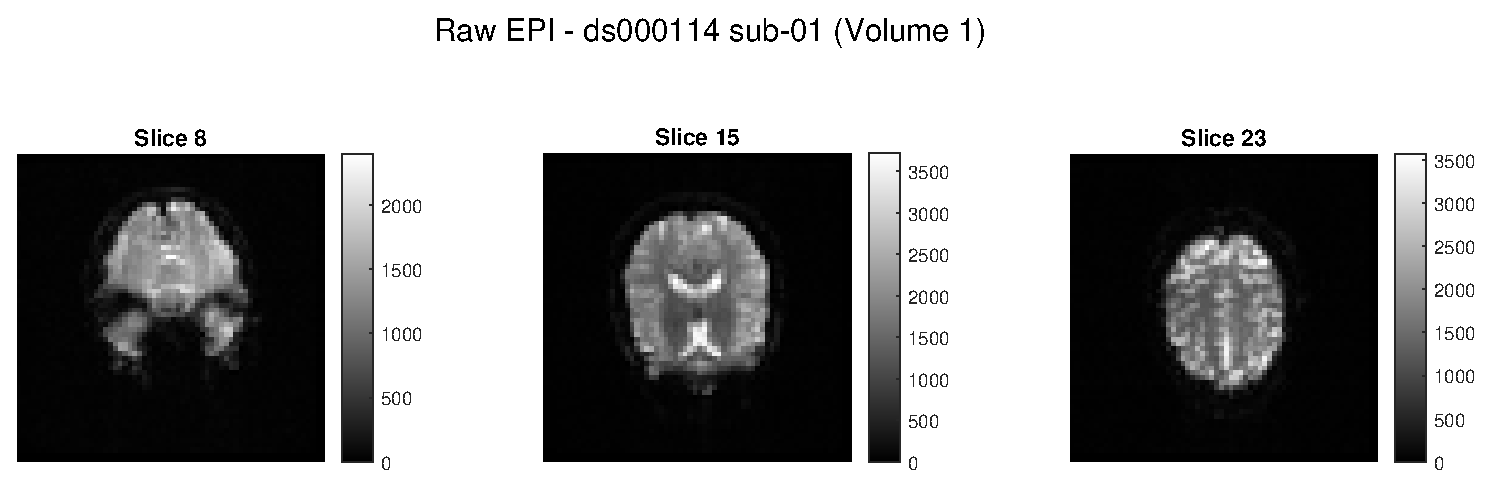
\includegraphics[width=\textwidth]{figures/fig01_ds1_raw_epi_sample}
  \caption{Raw EPI sample for Dataset~1 (ds000114, subject sub-01)
    before any preprocessing. Three axial slices at 25\%, 50\%, and
    75\% of the brain volume are shown. Signal dropout near the
    orbito-frontal cortex and temporal poles is characteristic of
    single-shot EPI at this field strength.}
  \label{fig:ds1:raw_epi}
\end{figure}

\begin{figure}[H]
  \centering
  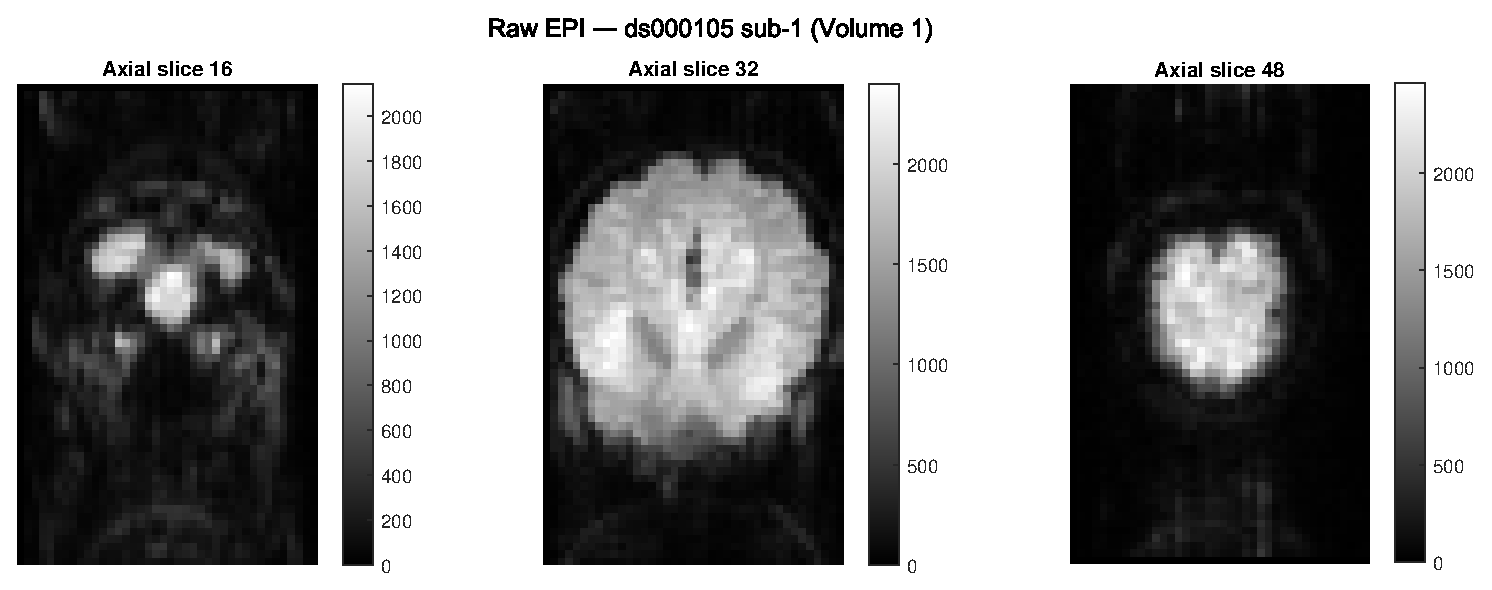
\includegraphics[width=\textwidth]{figures/fig06_ds2_raw_epi_sample}
  \caption{Raw EPI sample for Dataset~2 (ds000105, subject sub-1).
    The larger matrix size relative to Dataset~1 is apparent from
    the finer spatial detail, though EPI-related distortion near
    air-tissue boundaries remains visible.}
  \label{fig:ds2:raw_epi}
\end{figure}

\begin{figure}[H]
  \centering
  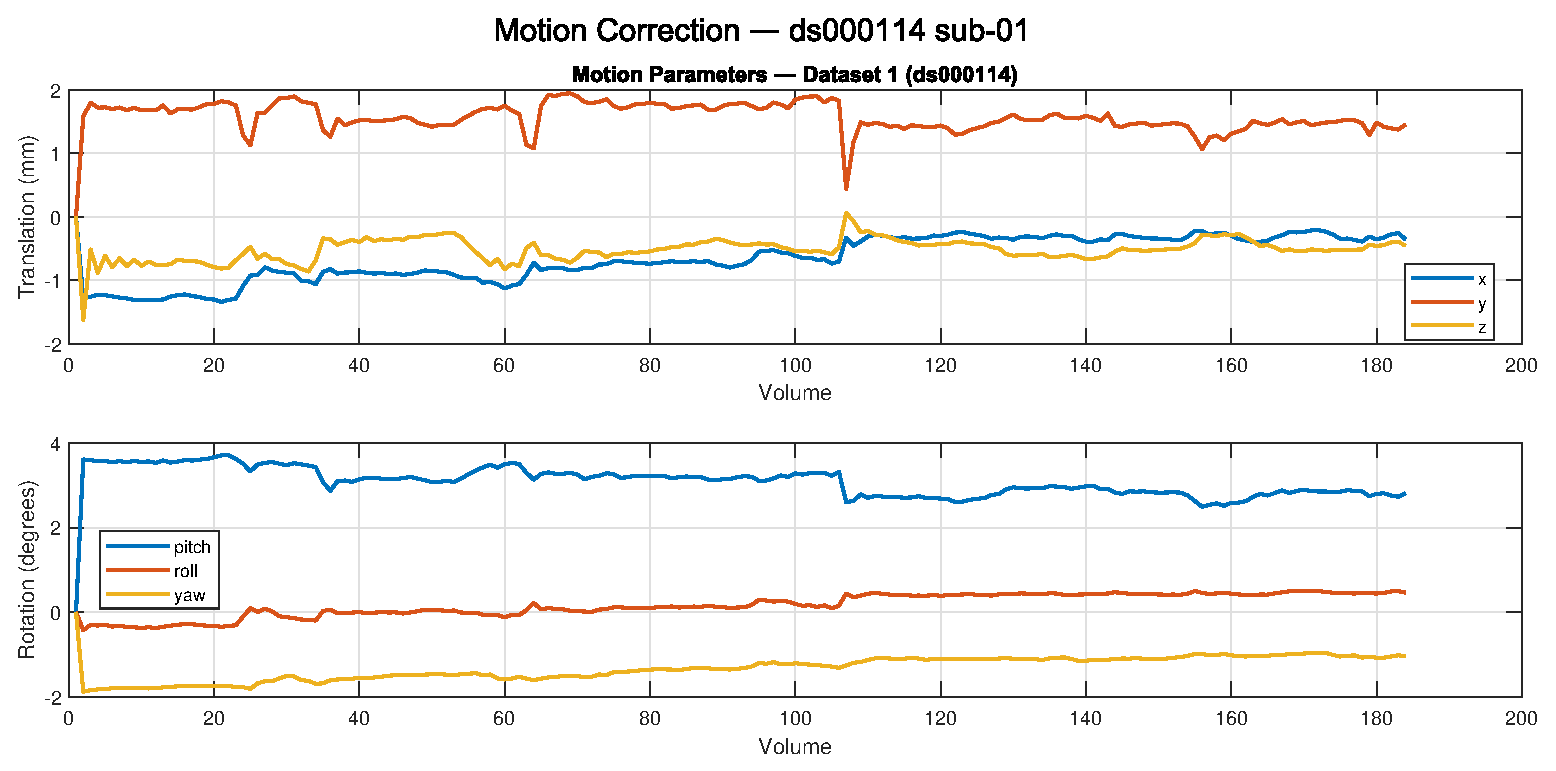
\includegraphics[width=\textwidth]{figures/fig02_ds1_motion_parameters}
  \caption{Head-motion parameters for Dataset~1 across all 184
    volumes. Top: three translational parameters (mm) along the
    right--left (x), anterior--posterior (y), and
    superior--inferior (z) axes. Bottom: three rotational parameters
    (degrees). Motion remains well below 1\,mm and 1$^\circ$
    throughout the scan.}
  \label{fig:ds1:motion_params}
\end{figure}

\begin{figure}[H]
  \centering
  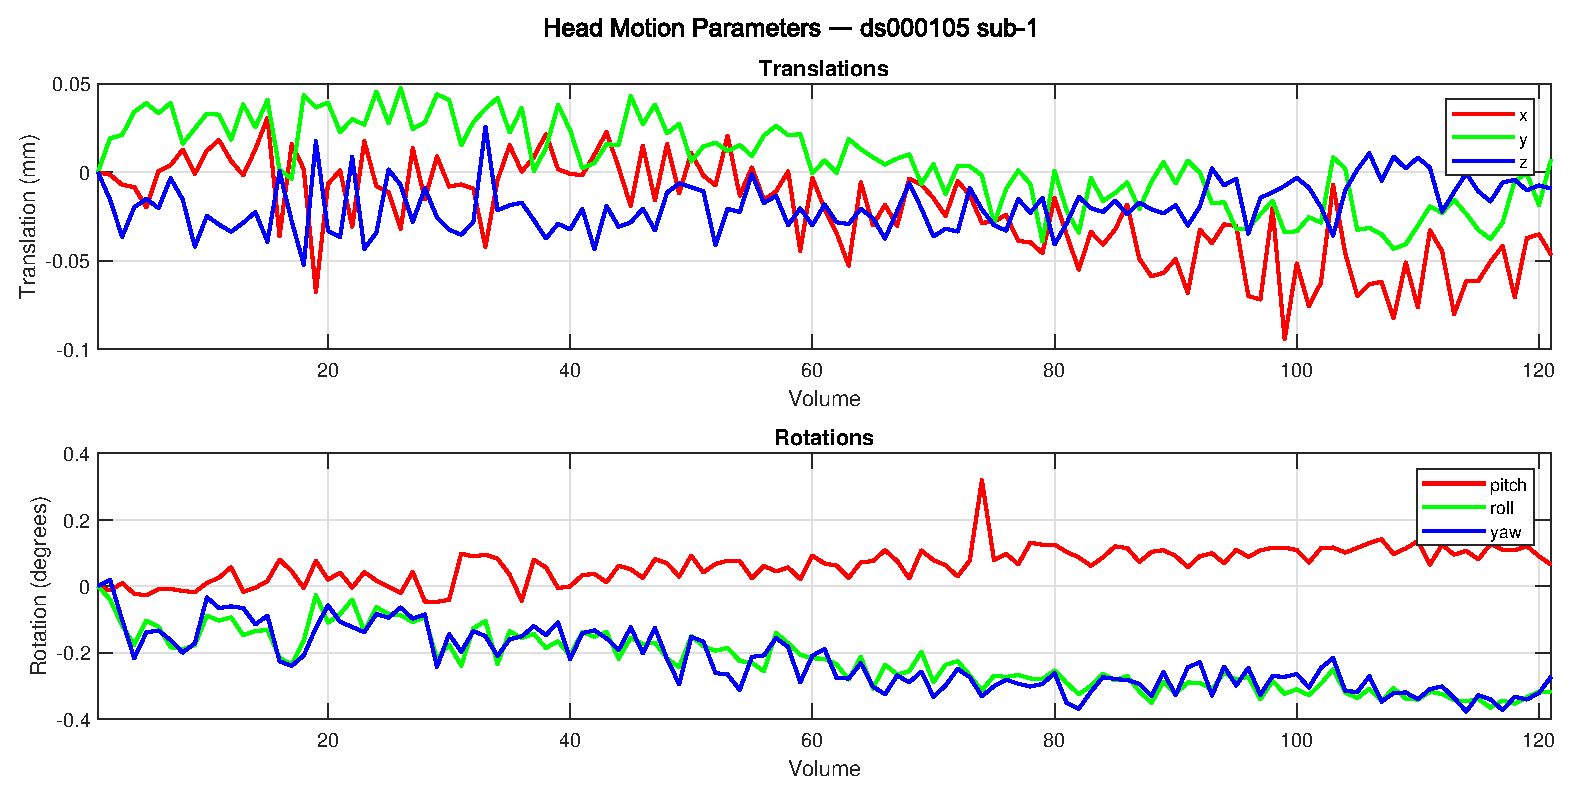
\includegraphics[width=\textwidth]{figures/fig07_ds2_motion_parameters}
  \caption{Head-motion parameters for Dataset~2 (121 volumes).
    The pattern is similarly low-amplitude, confirming that both
    subjects cooperated well during scanning.}
  \label{fig:ds2:motion_params}
\end{figure}

\textbf{Step 3 — Coregistration.}
Functional and anatomical images are acquired with different pulse
sequences and have different spatial resolutions, so they do not
naturally line up. Coregistration estimates the rigid-body
transformation that maximises normalised mutual information (NMI)
between the mean EPI image and the T1-weighted anatomical scan.
Once estimated, the same transformation is applied to all functional
volumes. The quality of alignment was checked visually by overlaying
the mean EPI on the T1 (Figs.~\ref{fig:ds1:coregistration}
and~\ref{fig:ds2:coregistration}).

\begin{figure}[H]
  \centering
  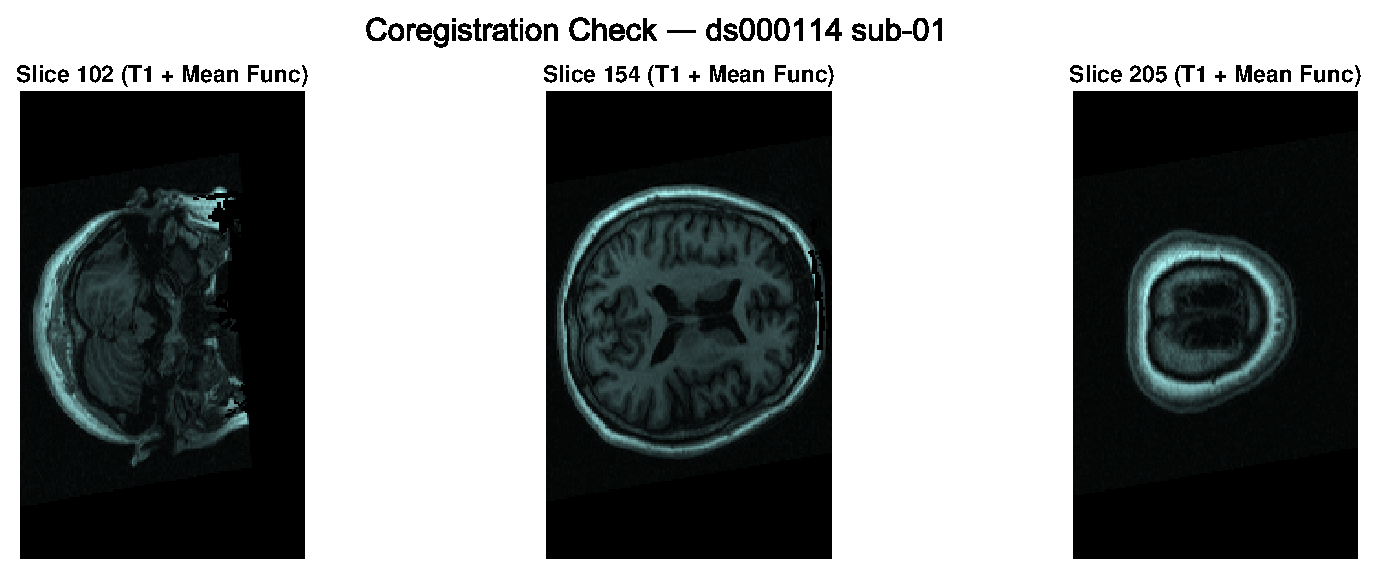
\includegraphics[width=\textwidth]{figures/fig03_ds1_coregistration}
  \caption{Coregistration quality check for Dataset~1. The T1
    anatomical image is shown in greyscale; the mean EPI is
    overlaid in red. Brain boundaries match well across the
    three axial slices, indicating successful coregistration.}
  \label{fig:ds1:coregistration}
\end{figure}

\begin{figure}[H]
  \centering
  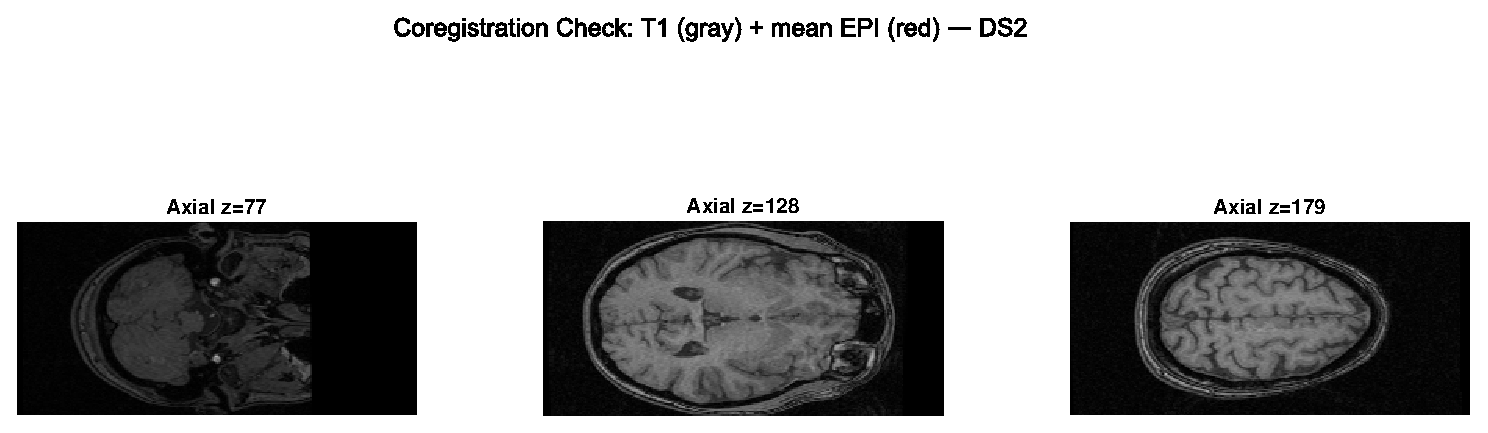
\includegraphics[width=\textwidth]{figures/fig08_ds2_coregistration}
  \caption{Coregistration check for Dataset~2. Same colour scheme
    as Fig.~\ref{fig:ds1:coregistration}. The alignment is
    anatomically consistent across the displayed slices.}
  \label{fig:ds2:coregistration}
\end{figure}

\textbf{Step 4 — Unified Segmentation.}
SPM's unified segmentation model~\cite{Ashburner2005} simultaneously
segments the T1 image into six tissue classes (grey matter, white
matter, CSF, bone, soft tissue, and background) and estimates the
non-linear deformation field ($y_*$) that maps the subject's brain
into MNI152 standard space. Running segmentation and normalisation
in a single model is more accurate than doing them sequentially,
because the tissue priors constrain the deformation.

\textbf{Step 5 — Normalisation.}
The deformation field from Step~4 is applied to write both the
functional volumes and the anatomical image into 2\,mm isotropic
MNI space (bounding box $[-78, -112, -70]$ to $[78, 76, 85]$\,mm).
After this step, every voxel has a known location in standard
space, making the results interpretable against the neuroimaging
literature. Temporal SNR maps computed before and after normalisation
are shown in Figs.~\ref{fig:ds1:tsnr_norm}
and~\ref{fig:ds2:tsnr_norm}.

\begin{figure}[H]
  \centering
  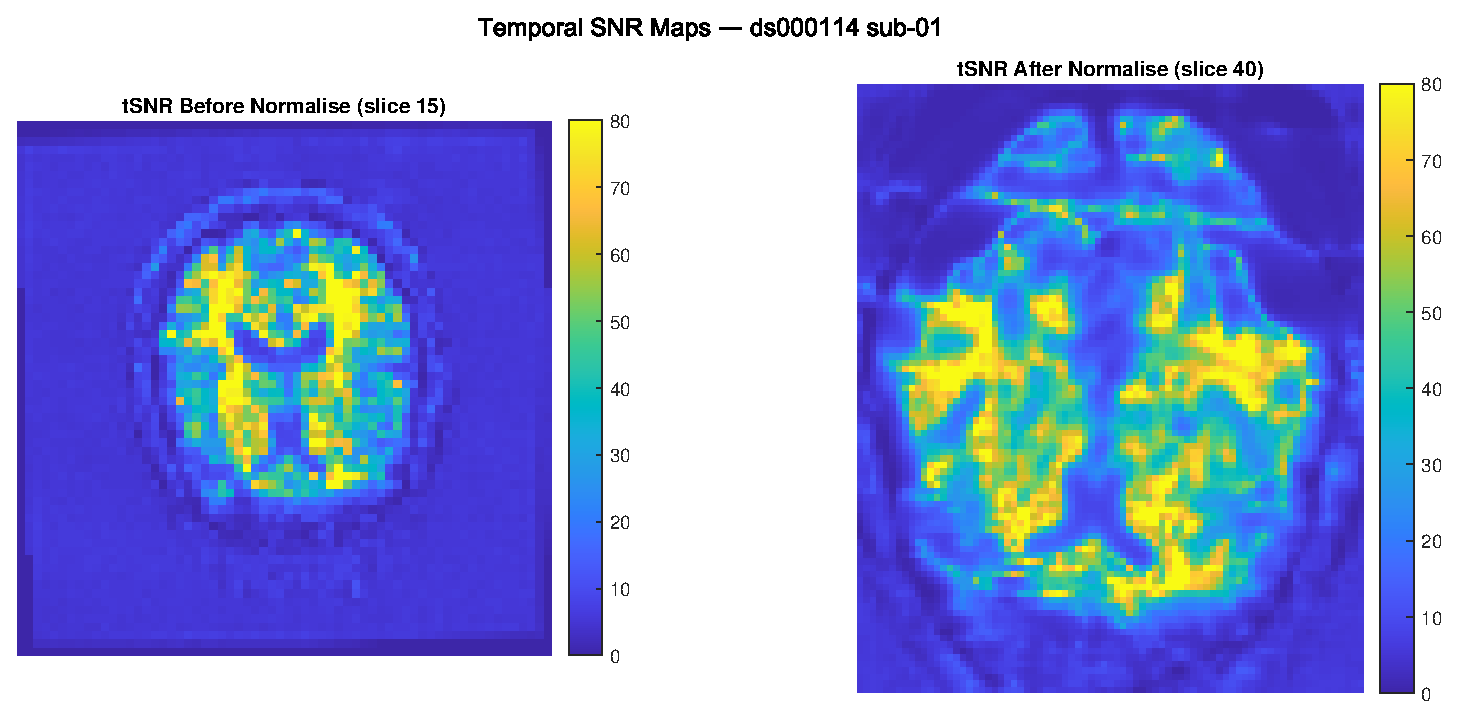
\includegraphics[width=\textwidth]{figures/fig04_ds1_tsnr_comparison}
  \caption{Temporal SNR at mid-brain axial slice for Dataset~1,
    before (left) and after (right) MNI normalisation. The overall
    tSNR level is maintained after the resampling step, with warm
    colours indicating higher signal stability.}
  \label{fig:ds1:tsnr_norm}
\end{figure}

\begin{figure}[H]
  \centering
  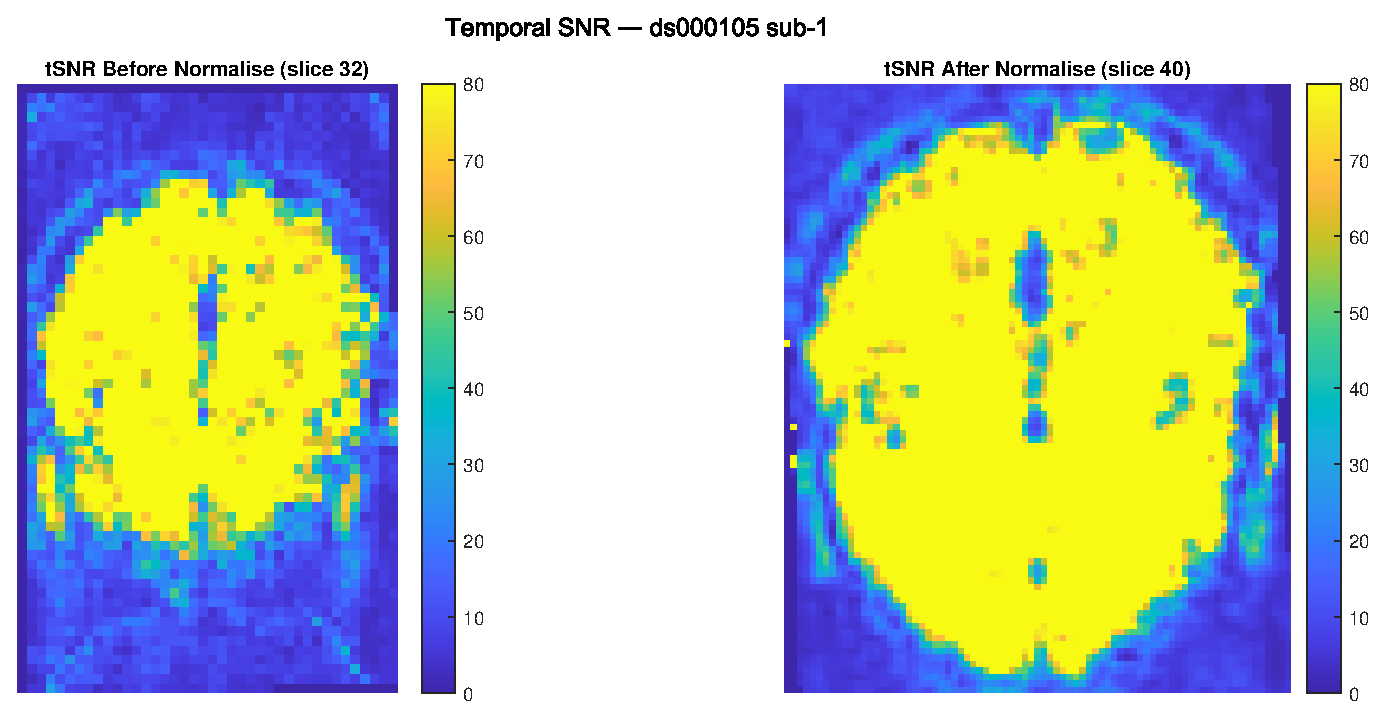
\includegraphics[width=\textwidth]{figures/fig09_ds2_tsnr_comparison}
  \caption{Temporal SNR for Dataset~2 before and after normalisation,
    shown at the same axial position as Fig.~\ref{fig:ds1:tsnr_norm}.
    The tSNR distribution is consistent with typical task-fMRI data.}
  \label{fig:ds2:tsnr_norm}
\end{figure}

\textbf{Step 6 — Spatial Smoothing.}
A 6\,mm isotropic Gaussian kernel is applied to the normalised
functional data. Smoothing increases SNR by averaging correlated
nearby voxels, helps normalise the residual error distribution (a
requirement for valid SPM statistics), and partially compensates for
residual anatomical differences between subjects. The cost is a
reduction in effective spatial resolution. Figures~\ref{fig:ds1:smoothing}
and~\ref{fig:ds2:smoothing} show how tSNR changes after smoothing.

\begin{figure}[H]
  \centering
  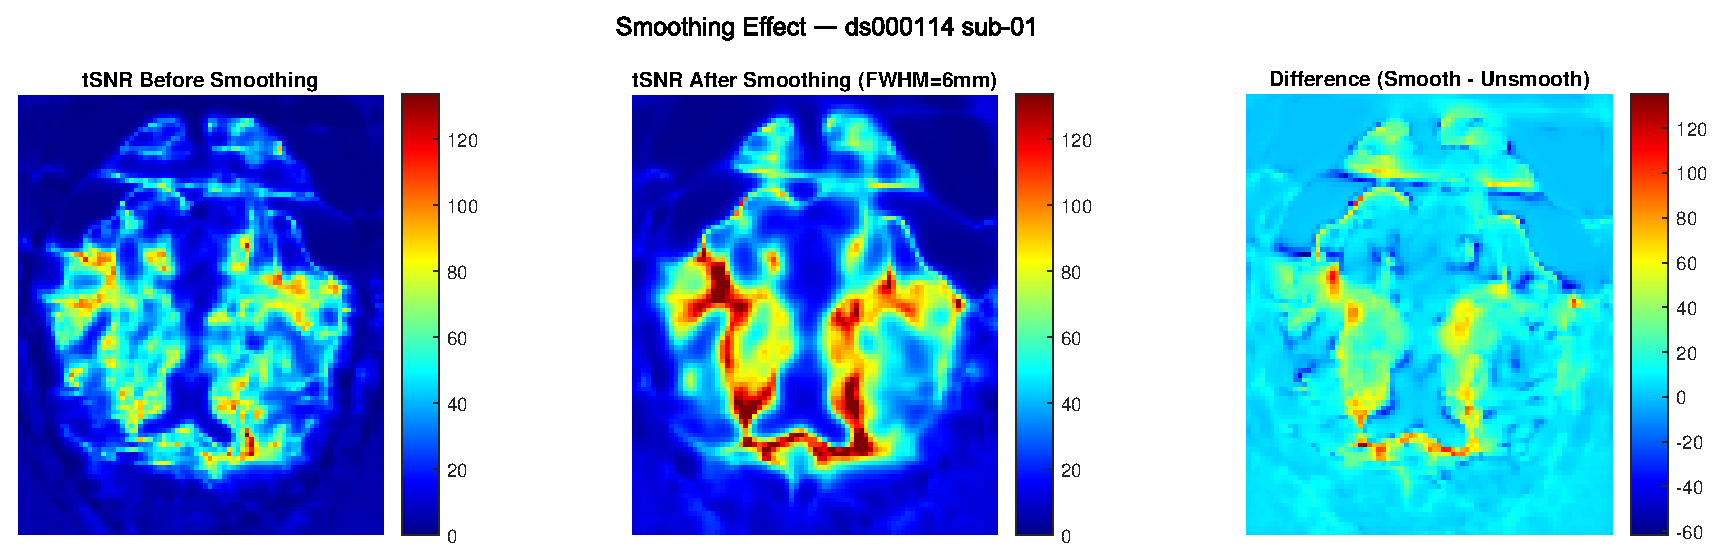
\includegraphics[width=\textwidth]{figures/fig05_ds1_smoothing_effect}
  \caption{Effect of 6\,mm Gaussian smoothing on temporal SNR for
    Dataset~1. Left: tSNR before smoothing. Centre: tSNR after
    smoothing. Right: difference map, where positive values (warm)
    indicate SNR gain. The improvement is broad and spatially
    uniform.}
  \label{fig:ds1:smoothing}
\end{figure}

\begin{figure}[H]
  \centering
  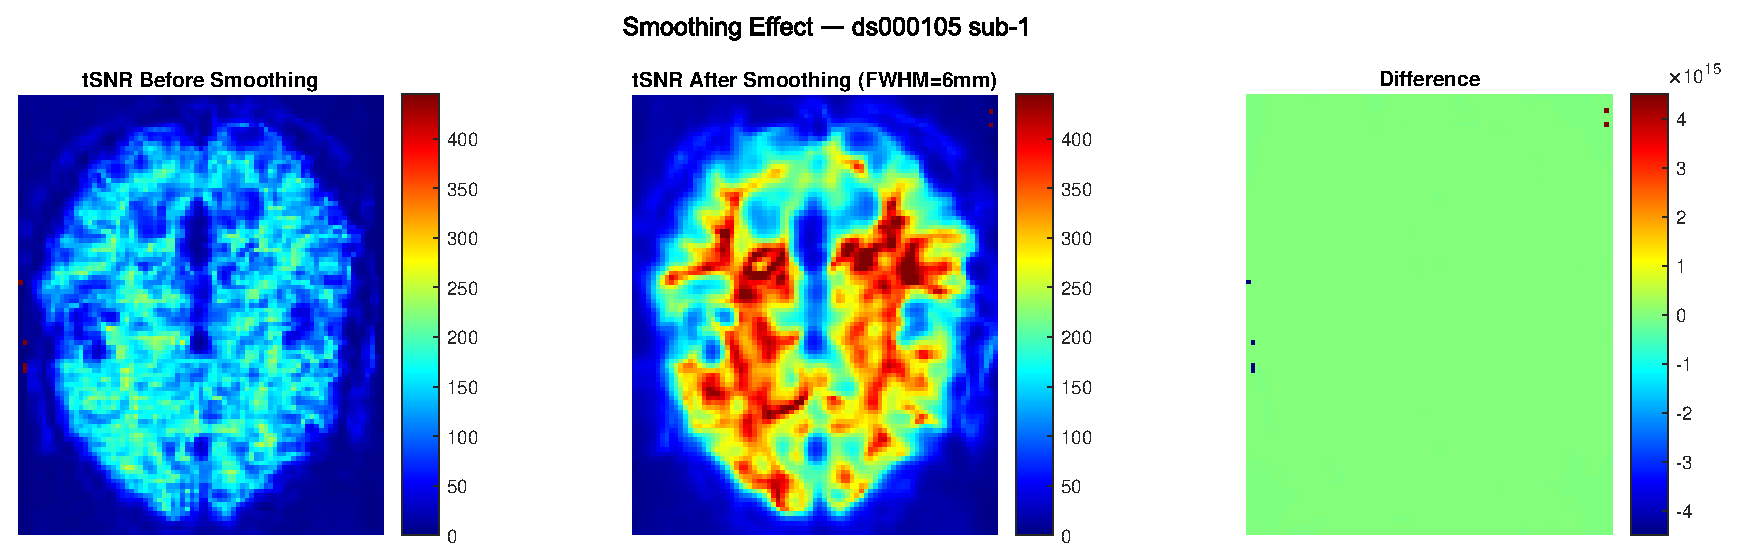
\includegraphics[width=\textwidth]{figures/fig10_ds2_smoothing_effect}
  \caption{Smoothing effect for Dataset~2, laid out identically to
    Fig.~\ref{fig:ds1:smoothing}. The SNR gain pattern is
    comparable across both datasets, confirming that neither
    acquisition was anomalously noisy.}
  \label{fig:ds2:smoothing}
\end{figure}

\subsection{General Linear Model}

The GLM was specified in SPM25 using the canonical double-gamma
haemodynamic response function (HRF) with no temporal or dispersion
derivatives~\cite{Friston1998}. Condition onsets and durations came
from the BIDS-formatted \texttt{events.tsv} files bundled with each
dataset. Each unique condition label became one column in the design
matrix, convolved with the HRF. Six motion parameters (from Step~2)
were added as additional columns to capture residual motion-related
variance. A 128\,s high-pass filter (implemented as a discrete
cosine transform basis set) removed slow scanner drifts, and
temporal autocorrelation was modelled with AR(1).

The timing structures of the two experiments are visualised in
Figs.~\ref{fig:ds1:design_timing} and~\ref{fig:ds2:design_timing},
and the resulting SPM design matrices are in
Figs.~\ref{fig:ds1:design_matrix} and~\ref{fig:ds2:design_matrix}.

\begin{figure}[H]
  \centering
  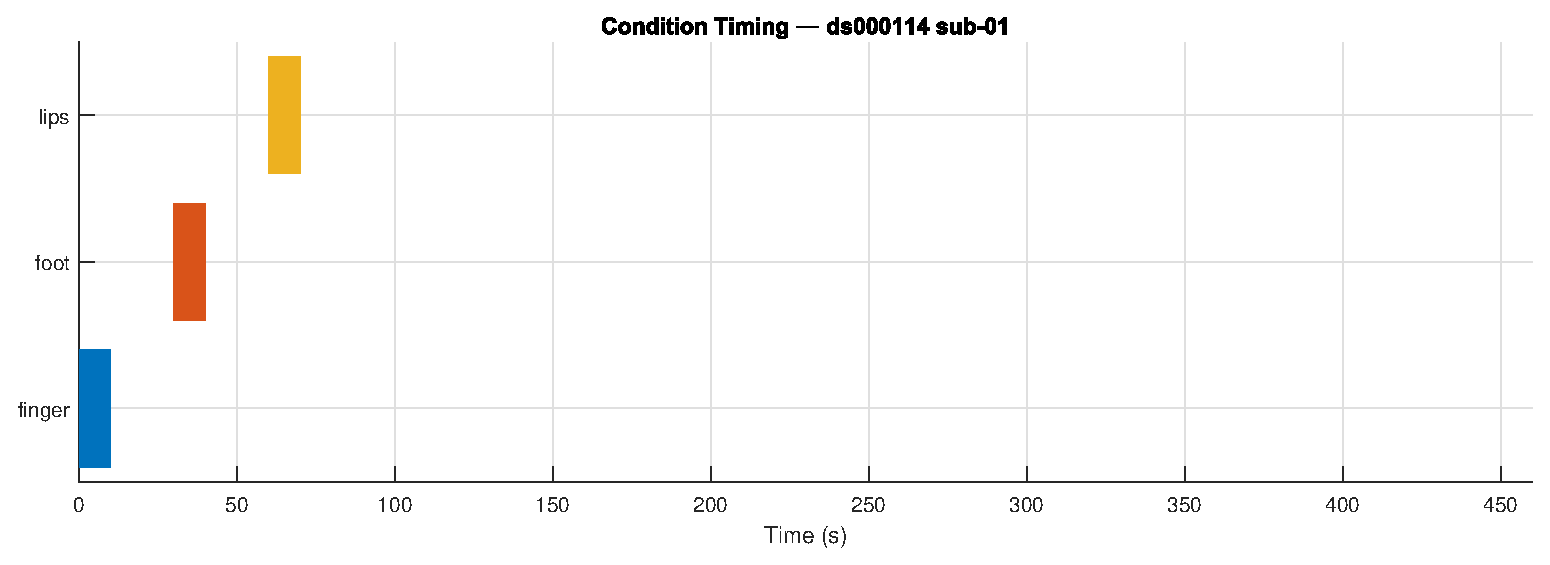
\includegraphics[width=\textwidth]{figures/fig11_ds1_design_timing}
  \caption{Experimental condition timing for Dataset~1 (ds000114).
    Each coloured bar represents one block of the motor task.
    The three conditions (foot, finger, lips) alternate with
    rest/instruction periods throughout the 460\,s run.}
  \label{fig:ds1:design_timing}
\end{figure}

\begin{figure}[H]
  \centering
  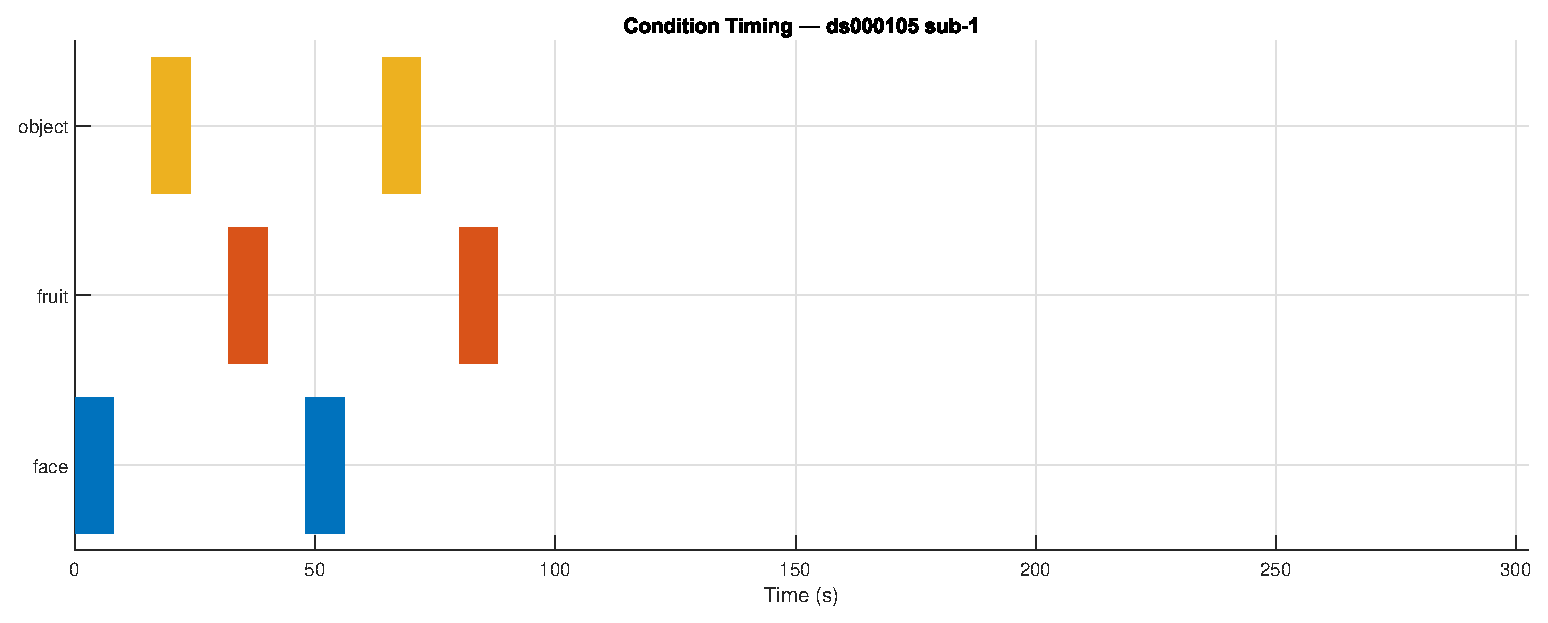
\includegraphics[width=\textwidth]{figures/fig17_ds2_design_timing}
  \caption{Condition timing for Dataset~2 (ds000105). Each row
    corresponds to one visual category. The design is event-related,
    with short stimulus presentations interleaved across the run.}
  \label{fig:ds2:design_timing}
\end{figure}

\begin{figure}[H]
  \centering
  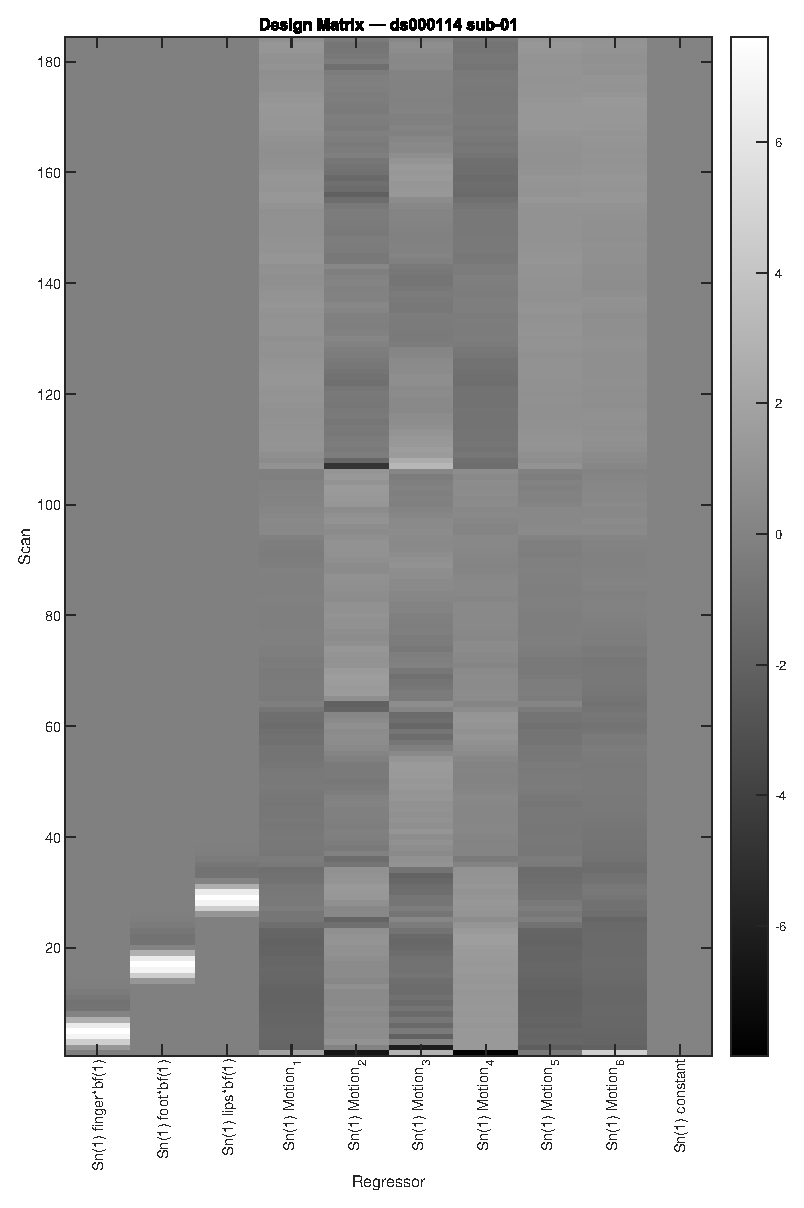
\includegraphics[width=0.75\textwidth]{figures/fig12_ds1_design_matrix}
  \caption{SPM design matrix for Dataset~1. Each column is one
    regressor (z-scored for display). The first columns are the
    HRF-convolved task regressors; the last six columns are the
    motion parameters. The block structure of the motor task is
    clearly visible.}
  \label{fig:ds1:design_matrix}
\end{figure}

\begin{figure}[H]
  \centering
  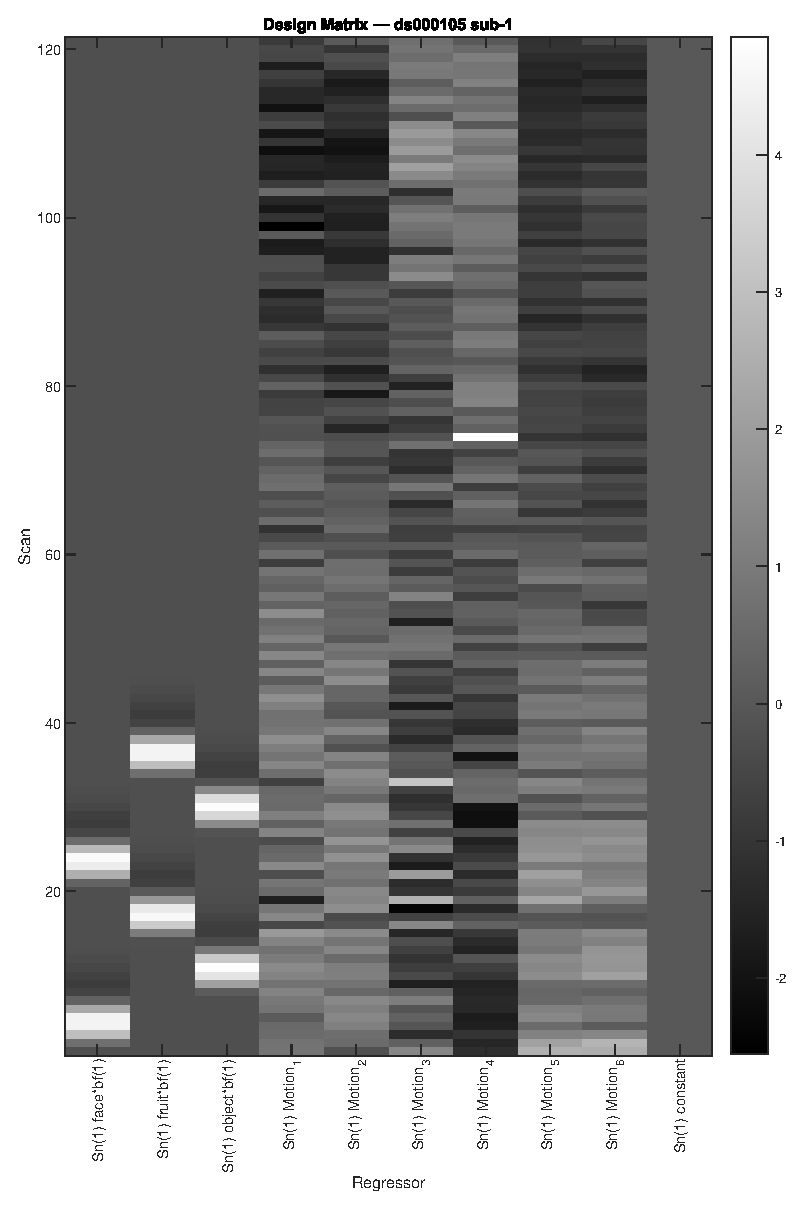
\includegraphics[width=0.75\textwidth]{figures/fig18_ds2_design_matrix}
  \caption{SPM design matrix for Dataset~2. The denser regressor
    pattern reflects the event-related nature of the visual task,
    where multiple short-duration trials overlap in time.}
  \label{fig:ds2:design_matrix}
\end{figure}

\textbf{Contrasts for Dataset~1 (Motor Task).}
Individual t-contrasts were defined for each motor condition against
implicit baseline (Finger$\,{>}\,$Baseline, Foot$\,{>}\,$Baseline,
Lips$\,{>}\,$Baseline) and an omnibus contrast pooling all three
conditions (AllMotor$\,{>}\,$Baseline). An F-test served as an
unbiased overall test of motor activity.

\textbf{Contrasts for Dataset~2 (Visual Task).}
One t-contrast per visual category tested activation against
implicit baseline. Where a scrambled-image condition was present,
additional contrasts of the form Category$\,{>}\,$Scrambled were
computed to isolate category-specific processing from general
low-level visual responses.

All maps were thresholded at $p<0.001$ uncorrected with a minimum
cluster extent of $k>10$ voxels.

\subsection{Functional Connectivity}

Seed-based connectivity was computed directly from the preprocessed
time series. A 6\,mm-radius spherical ROI was centred on:
\begin{itemize}
  \item \textbf{Dataset~1}: Left primary motor cortex (M1) at MNI
        $[-38, -26, 60]$\,mm, a well-established hand-area
        coordinate~\cite{Biswal1995}.
  \item \textbf{Dataset~2}: Primary visual cortex (V1) at MNI
        $[0, -88, 2]$\,mm, within the calcarine sulcus.
\end{itemize}
The mean signal across all seed voxels was extracted, then high-pass
filtered at 0.01\,Hz to remove very slow drifts. Pearson correlation
coefficients between this seed time series and every other brain voxel
were computed, then Fisher $z$-transformed to stabilise variance:
\begin{equation}
  z(r) = \tanh^{-1}(r) =
  \frac{1}{2}\ln\!\left(\!\frac{1+r}{1-r}\!\right).
\end{equation}
Resulting $z$-maps were thresholded at $r > 0.30$ for display
purposes.

